\begin{chapterenv}

\chapter{Direct Preference Optimization}

\section{From RLHF to DPO}

Chapter 6 revealed both the power and the pain of classical RLHF. The power: a reward model trained on human comparisons can guide a policy to produce responses that are better than anything in its original training data. The pain: you need four models in GPU memory simultaneously, PPO has a dozen sensitive hyperparameters, and the reward model itself can be exploited through reward hacking.

In 2023, Rafael Rafailov and colleagues at Stanford asked a deceptively simple question: \textit{what if we could skip the reward model entirely?} Their paper, ``Direct Preference Optimization: Your Language Model Is Secretly a Reward Model,'' showed that the answer was yes. The mathematical insight is elegant: the reward function that the RLHF pipeline learns is already encoded, implicitly, inside the policy itself. You do not need to extract it into a separate model. You can train the policy directly on preference pairs, with no reward model, no value function, no PPO loop.

The result is DPO: a method that achieves comparable performance to full RLHF while cutting memory requirements in half and replacing a complex RL training loop with something that looks almost like supervised learning. This chapter derives DPO from the ground up, walks through the math with concrete numbers, and explains when DPO is the right choice and when it is not.

\section{The Reparameterization Trick}

The derivation starts from the same place as Chapter 6: the Bradley-Terry model of preferences and the KL-constrained reward maximization objective. Recall the RLHF objective from Section 6.3.1:

$$\max_{\pi_\theta} \; \mathbb{E}_{x,y}\!\left[r_\phi(x,y)\right] - \beta \cdot \mathbb{E}_x\!\left[\text{KL}(\pi_\theta \,\|\, \pi_{\text{ref}})\right]$$

This objective has a known closed-form solution. If you could solve it perfectly, the optimal policy $\pi^*$ would take a specific mathematical form. DPO's insight is to write down that form, rearrange it, and substitute back into the Bradley-Terry preference model from Section 6.2.2. When you do, something remarkable happens: the reward model cancels out entirely.

\textbf{The DPO Reparameterization in Three Steps}

\begin{infobox}
\textbf{Step 1: Write down the optimal policy}

$$\pi^*(y|x) = \frac{1}{Z(x)}\, \pi_{\text{ref}}(y|x)\, \exp\!\left(\frac{r(x,y)}{\beta}\right)$$

The best possible policy takes the reference model and reweights each response by the exponential of its reward. $Z(x)$ is a normalizing constant that ensures probabilities sum to 1.
\end{infobox}

\begin{infobox}
\textbf{Step 2: Solve for the reward}

$$r(x,y) = \beta \log \frac{\pi^*(y|x)}{\pi_{\text{ref}}(y|x)} + \beta \log Z(x)$$

Rearranging Step 1 gives us the reward as a function of the policy ratio. The reward for any response is proportional to how much more likely the optimal policy makes it compared to the reference.
\end{infobox}

\begin{infobox}
\textbf{Step 3: Substitute into Bradley-Terry}

$$P(y_w \succ y_l) = \sigma\!\left(\beta \log \frac{\pi(y_w|x)}{\pi_{\text{ref}}(y_w|x)} - \beta \log \frac{\pi(y_l|x)}{\pi_{\text{ref}}(y_l|x)}\right)$$

When we plug the reward expression into the preference model from Chapter 6, the partition function $Z(x)$ appears in both terms and cancels. We are left with preference probability expressed entirely in terms of policy ratios. No reward model anywhere.
\end{infobox}

\textbf{Why does $Z(x)$ cancel?} In the Bradley-Terry model, the preference probability depends on the \textit{difference} between the rewards for the winner and loser: $r(x, y_w) - r(x, y_l)$. When we substitute the Step 2 expression for both rewards, each contains the same $\beta \log Z(x)$ term. Subtracting one from the other eliminates $Z(x)$ completely. This is the mathematical core of DPO: a term that would be intractable to compute simply drops out of the equation.

\textbf{What this means in practice.} Recall from Chapter 6 that RLHF requires four models: the policy, the reference, the reward model, and the value function. The reparameterization trick shows that we can express the preference probability using only the policy and the reference. The reward model and value function are no longer needed.

\begin{center}
\begin{tabular}{lcc}
\toprule
\textbf{Component} & \textbf{RLHF (Chapter 6)} & \textbf{DPO} \\
\midrule
Policy $\pi_\theta$ & Yes (trainable) & Yes (trainable) \\
Reference $\pi_{\text{ref}}$ & Yes (frozen) & Yes (frozen) \\
Reward model $r_\phi$ & Yes (frozen) & \textbf{Not needed} \\
Value function $V$ & Yes (trainable) & \textbf{Not needed} \\
\midrule
\textbf{Total models} & 4 & 2 \\
\bottomrule
\end{tabular}
\end{center}

\begin{infobox}
\textbf{The key insight.} We do not need to explicitly model the reward function $r(x,y)$. The policy ratio $\frac{\pi_\theta(y|x)}{\pi_{\text{ref}}(y|x)}$ already encodes all the information about what makes responses good.

If $\pi_\theta$ makes a response more likely than $\pi_{\text{ref}}$ does, that response has high \textit{implicit} reward. If $\pi_\theta$ makes it less likely, the response has low implicit reward. Training can adjust $\pi_\theta$ directly on preference pairs, without ever computing an explicit reward score.
\end{infobox}

\section{The DPO Loss Function}

The reparameterization gives us a way to express preference probability in terms of policy ratios. To turn this into a training objective, we apply maximum likelihood: find the policy parameters $\theta$ that make the observed preference data most likely.

\begin{infobox}
\textbf{Training the Policy Directly on Preferences}

$$\mathcal{L}_{\text{DPO}}(\theta) = -\mathbb{E}\!\left[\log \sigma\!\left(\beta \log \frac{\pi_\theta(y_w|x)}{\pi_{\text{ref}}(y_w|x)} - \beta \log \frac{\pi_\theta(y_l|x)}{\pi_{\text{ref}}(y_l|x)}\right)\right]$$

\textbf{In plain English:} Adjust the policy so that for every preference pair, the winner's implicit reward is higher than the loser's.
\end{infobox}

\textbf{Breaking it apart:}

\begin{center}
\begin{tabular}{p{0.35\textwidth}p{0.55\textwidth}}
\toprule
\textbf{Component} & \textbf{Purpose} \\
\midrule
$\beta \log \frac{\pi_\theta(y_w|x)}{\pi_{\text{ref}}(y_w|x)}$ & Implicit reward for the winner. How much has the policy increased the winner's likelihood relative to the reference? \\
$\beta \log \frac{\pi_\theta(y_l|x)}{\pi_{\text{ref}}(y_l|x)}$ & Implicit reward for the loser. How much has the policy increased the loser's likelihood relative to the reference? \\
$\sigma(\text{winner} - \text{loser})$ & Probability that the policy assigns higher implicit reward to the winner than the loser. Should be close to 1 if training is working. \\
$\log(\cdot)$ & Log likelihood. Heavily penalizes confident wrong predictions (when the model thinks the loser is better). \\
$-$ & Flip sign so that minimizing the loss maximizes correct preference predictions. \\
$\mathbb{E}[\cdot]$ & Average over all preference pairs in the dataset. \\
\bottomrule
\end{tabular}
\end{center}

\begin{infobox}
\textbf{Compare with the reward model loss from Chapter 6:}

\textbf{Reward model loss (Chapter 6):}
$$-\mathbb{E}\!\left[\log \sigma\!\left(r_\phi(x, y_w) - r_\phi(x, y_l)\right)\right]$$

\textbf{DPO loss (this chapter):}
$$-\mathbb{E}\!\left[\log \sigma\!\left(\beta \log \frac{\pi_\theta(y_w|x)}{\pi_{\text{ref}}(y_w|x)} - \beta \log \frac{\pi_\theta(y_l|x)}{\pi_{\text{ref}}(y_l|x)}\right)\right]$$

The structure is identical. The only difference is what plays the role of the ``score'': explicit reward model outputs $r_\phi$ in RLHF, versus implicit rewards from policy ratios $\beta \log \frac{\pi_\theta}{\pi_{\text{ref}}}$ in DPO. Same framework, different parameterization.
\end{infobox}

\section{Step-by-Step Walkthrough}

Let us trace through DPO training on a single preference pair, computing every number.

\textbf{Preference pair:}
\begin{itemize}[nosep]
    \item \textbf{Prompt ($x$):} ``Explain photosynthesis''
    \item \textbf{Winner ($y_w$):} ``Plants use sunlight to make food from CO$_2$ and water'' (10 tokens)
    \item \textbf{Loser ($y_l$):} ``Photosynthesis is the biochemical process involving chloroplast thylakoids\ldots'' (12 tokens)
\end{itemize}

The winner is simpler and clearer. We want DPO to learn this preference.

\paragraph{Step 1: Compute token probabilities for both responses}

For each response, both the current policy $\pi_\theta$ and the frozen reference $\pi_{\text{ref}}$ assign a probability to every token. For simplicity, we use average per-token probabilities.

\textbf{Winner (10 tokens):}

\begin{center}
\begin{tabular}{lcc}
\toprule
\textbf{Model} & \textbf{Avg per-token probability} & \textbf{Full sequence probability} \\
\midrule
$\pi_\theta$ (current) & 0.22 & $0.22^{10}$ \\
$\pi_{\text{ref}}$ (reference) & 0.20 & $0.20^{10}$ \\
\bottomrule
\end{tabular}
\end{center}

\textbf{Loser (12 tokens):}

\begin{center}
\begin{tabular}{lcc}
\toprule
\textbf{Model} & \textbf{Avg per-token probability} & \textbf{Full sequence probability} \\
\midrule
$\pi_\theta$ (current) & 0.17 & $0.17^{12}$ \\
$\pi_{\text{ref}}$ (reference) & 0.19 & $0.19^{12}$ \\
\bottomrule
\end{tabular}
\end{center}

Notice what is already happening: the current policy assigns slightly higher probability to each winner token (0.22 vs 0.20) and slightly lower probability to each loser token (0.17 vs 0.19) compared to the reference. The policy is starting to differentiate, but only slightly.

\paragraph{Step 2: Compute log ratios (the implicit rewards)}

\textbf{Winner log ratio:}
\begin{align*}
\log \frac{\pi_\theta(y_w|x)}{\pi_{\text{ref}}(y_w|x)} &= 10 \times \log \frac{0.22}{0.20} = 10 \times 0.095 = 0.95
\end{align*}

The current policy makes the winner 0.95 log-units more likely than the reference does. This is a positive implicit reward: the policy ``likes'' this response.

\textbf{Loser log ratio:}
\begin{align*}
\log \frac{\pi_\theta(y_l|x)}{\pi_{\text{ref}}(y_l|x)} &= 12 \times \log \frac{0.17}{0.19} = 12 \times (-0.111) = -1.33
\end{align*}

The current policy makes the loser 1.33 log-units \textit{less} likely than the reference. Negative implicit reward: the policy has already started moving away from this response.

\paragraph{Step 3: Compute the preference logit}

With $\beta = 0.1$:

\begin{align*}
\text{logit} &= \beta \times \left(\text{winner log ratio} - \text{loser log ratio}\right) \\
&= 0.1 \times \left(0.95 - (-1.33)\right) \\
&= 0.1 \times 2.28 = 0.228
\end{align*}

\paragraph{Step 4: Convert to preference probability}

\begin{align*}
P(\text{winner} \succ \text{loser}) &= \sigma(0.228) = \frac{1}{1 + e^{-0.228}} = 0.557 \quad \text{or } 55.7\%
\end{align*}

The model is only slightly better than chance at distinguishing the winner from the loser. Not great yet.

\paragraph{Step 5: Compute the loss}

\begin{align*}
\mathcal{L}_{\text{DPO}} &= -\log(0.557) = 0.585
\end{align*}

Recall from Chapter 6 that a random model produces a loss of $-\log(0.5) = 0.693$. Our loss of 0.585 is only slightly better than random, confirming that the model has barely begun to learn this preference.

\paragraph{Step 6: Gradient descent updates $\pi_\theta$}

The gradients push in two directions simultaneously. They \textbf{increase} $\pi_\theta(y_w|x)$, making the winner tokens more likely under the policy. And they \textbf{decrease} $\pi_\theta(y_l|x)$, making the loser tokens less likely. This is the core learning dynamic of DPO: every preference pair teaches the model to widen the gap between winner-style and loser-style responses.

\paragraph{After training on 50,000 preference pairs}

Running the same computation on this preference pair after training:

\begin{center}
\begin{tabular}{lcc}
\toprule
\textbf{Quantity} & \textbf{Before training} & \textbf{After training} \\
\midrule
Winner log ratio & $+0.95$ & $+2.8$ \\
Loser log ratio & $-1.33$ & $-2.5$ \\
Difference & $2.28$ & $5.3$ \\
Logit ($\beta = 0.1$) & $0.228$ & $0.53$ \\
$P(\text{winner} \succ \text{loser})$ & 55.7\% & 62.9\% \\
Loss & 0.585 & 0.464 \\
\bottomrule
\end{tabular}
\end{center}

The model has learned to prefer simpler explanations, assign higher probability to clear and accessible language, and assign lower probability to overly technical responses. All of this happened without an explicit reward model. The policy learned directly from preference pairs.

\begin{infobox}
\textbf{Why DPO works.} Every preference pair teaches the model: ``This style of response is better than that style.'' The policy ratios $\frac{\pi_\theta}{\pi_{\text{ref}}}$ encode implicit rewards that are mathematically equivalent to the explicit rewards that a separate reward model would produce. Training automatically makes winner log ratios larger and loser log ratios smaller.

The training loop is remarkably simple: load a batch of preference pairs, compute log probabilities under $\pi_\theta$ and $\pi_{\text{ref}}$, compute the DPO loss, backpropagate. No generation step, no reward scoring, no advantage estimation, no PPO clipping. It looks and feels like supervised learning, but it optimizes the same objective as RLHF.
\end{infobox}

\section{DPO vs RLHF: A Head-to-Head Comparison}

Now that you understand both methods, let us compare them directly. The right choice depends on your specific constraints.

\begin{center}
\small
\begin{tabular}{p{0.22\textwidth}p{0.33\textwidth}p{0.33\textwidth}}
\toprule
\textbf{Dimension} & \textbf{RLHF with PPO (Chapter 6)} & \textbf{DPO (this chapter)} \\
\midrule
\textbf{Models in memory} & 4 (policy, reference, reward, value) & 2 (policy, reference) \\
\textbf{Training pipeline} & Three separate stages (SFT $\to$ reward model $\to$ PPO) & Two stages (SFT $\to$ DPO) \\
\textbf{Training stability} & Sensitive to many hyperparameters (clip range, PPO epochs, GAE $\lambda$, etc.) & Relatively stable; fewer hyperparameters to tune \\
\textbf{Data requirements} & Can generate new data on-the-fly (online) & Requires a fixed dataset of preference pairs (offline) \\
\textbf{Exploration} & Policy generates new responses each iteration; can discover novel strategies & No generation during training; limited to strategies present in the preference data \\
\textbf{Reward hacking} & Risk of exploiting reward model weaknesses; KL penalty helps but is imperfect & Different risk profile: can overfit to preference data artifacts instead \\
\textbf{Compute cost} & High (generation + scoring + RL updates per batch) & Lower (forward passes through two models, standard backprop) \\
\textbf{Implementation} & Complex (PPO loop, advantage estimation, multiple model synchronization) & Simple (looks like supervised fine-tuning with a modified loss) \\
\textbf{Peak performance} & Slightly higher ceiling with abundant compute and careful tuning & Comparable in most settings; may lag behind in high-compute regimes \\
\bottomrule
\end{tabular}
\end{center}

\textbf{When does RLHF still win?}

RLHF with PPO retains advantages in two scenarios. First, when you have abundant compute and engineering resources, PPO's online exploration can discover response strategies that are not present in any static preference dataset. The policy generates novel responses, the reward model scores them, and training reinforces whatever works. DPO cannot do this because it never generates responses during training.

Second, when the task distribution shifts between preference data collection and deployment, PPO adapts better because it continuously generates and evaluates responses from the current policy. DPO trains on a fixed dataset, so if that dataset does not cover the prompts the model will face in production, performance can degrade.

\textbf{When is DPO the better choice?}

For most practitioners, DPO is the pragmatic default. If you are working with limited GPU memory (a single consumer GPU or a free Colab T4), DPO's two-model footprint may be the only viable option. If you want a simpler, more reproducible training pipeline, DPO eliminates the complex PPO loop and its many hyperparameters. If you already have a good preference dataset (or can generate one synthetically using a stronger model), DPO can match RLHF performance with less effort.

\begin{tipbox}
\textbf{The practitioner's rule of thumb.} Start with DPO. It is simpler to implement, faster to iterate, and easier to debug. If you observe specific problems that DPO cannot solve (distribution mismatch, insufficient exploration, performance plateau), then consider the more complex alternatives: Online DPO (Chapter 8) adds exploration back, and PPO (Chapter 6) provides the full online RL loop.
\end{tipbox}

\pagebreak[3]
\section{The $\beta$ Parameter and Practical Considerations}

\subsection{Understanding $\beta$ in DPO}

In Chapter 6, $\beta$ appeared as the coefficient on the KL penalty in the RLHF objective. In DPO, $\beta$ appears in the loss function directly, but it plays an analogous role: it controls how far the policy is allowed to deviate from the reference model.

\textbf{Formally,} $\beta$ scales the log ratios in the DPO loss:

$$\mathcal{L}_{\text{DPO}} = -\mathbb{E}\!\left[\log \sigma\!\left(\beta \log \frac{\pi_\theta(y_w|x)}{\pi_{\text{ref}}(y_w|x)} - \beta \log \frac{\pi_\theta(y_l|x)}{\pi_{\text{ref}}(y_l|x)}\right)\right]$$

A larger $\beta$ amplifies the log ratios, making the loss more sensitive to small differences between the policy and reference. A smaller $\beta$ dampens the log ratios, allowing the policy to deviate further before the loss reacts.

\textbf{Effect of $\beta$ on the same preference pair:}

Using the log ratios from our photosynthesis example (winner: $+0.95$, loser: $-1.33$, difference: $2.28$):

\begin{center}
\begin{tabular}{ccccl}
\toprule
$\beta$ & \textbf{Logit} & $P(\text{w} \succ \text{l})$ & \textbf{Loss} & \textbf{Interpretation} \\
\midrule
0.01 & 0.023 & 50.6\% & 0.690 & Almost no signal. Policy barely distinguishes winner from loser. Loss is near random baseline (0.693). \\
0.05 & 0.114 & 52.8\% & 0.637 & Weak signal. Slow learning. \\
0.10 & 0.228 & 55.7\% & 0.585 & Moderate signal. Standard starting point. \\
0.20 & 0.456 & 61.2\% & 0.490 & Strong signal. Faster learning but more sensitivity. \\
0.50 & 1.140 & 75.8\% & 0.277 & Very strong signal. Risk of overfitting to noisy preferences. \\
\bottomrule
\end{tabular}
\end{center}

\begin{infobox}
\textbf{Tuning $\beta$ in DPO}

\textbf{Too small} ($\beta < 0.05$): The loss function is nearly flat. Gradients are tiny, learning is extremely slow, and the model may fail to converge. Equivalent to a very tight leash--the policy barely moves from the reference.

\textbf{Just right} ($\beta = 0.1$ to $0.2$): The standard range for most tasks. The loss provides clear gradients without being oversensitive to noise in the preference data. Start here.

\textbf{Too large} ($\beta > 0.5$): The loss reacts strongly to every preference pair, including noisy or mislabeled ones. The policy can overfit to artifacts in the data (such as preferring longer responses because annotators tended to pick longer answers). Equivalent to a loose leash--the policy drifts far from the reference.

\textbf{Relationship to Chapter 6:} In RLHF, $\beta$ controls the KL penalty strength. A large $\beta$ in RLHF means a tight leash (conservative policy). In DPO, the relationship is \textit{inverted}: a large $\beta$ amplifies the implicit reward signal, effectively giving the policy more room to move. This difference can be confusing when switching between the two frameworks, so be careful when reading papers that use both.
\end{infobox}

\subsection{Other Hyperparameters}

Beyond $\beta$, several practical choices affect DPO training quality.

\textbf{Learning rate.} DPO is more sensitive to learning rate than standard supervised fine-tuning. A rate that works well for SFT (e.g., $2 \times 10^{-5}$) is often too high for DPO. Typical starting points are $5 \times 10^{-7}$ to $5 \times 10^{-6}$. If the loss spikes or the model degenerates, reduce the learning rate first.

\textbf{Batch size.} Because DPO averages over preference pairs, larger batches give more stable gradient estimates. A batch size of 32 to 64 preference pairs is common. If you are memory-constrained, use gradient accumulation to simulate larger batches.

\textbf{Reference model handling.} The reference model $\pi_{\text{ref}}$ must remain fixed throughout training. In practice, this means loading a second copy of the SFT model in inference mode. With LoRA, you can share the base model weights and only keep separate adapter weights for $\pi_\theta$, which significantly reduces memory. Some implementations precompute $\pi_{\text{ref}}$'s log probabilities for all responses in the preference dataset before training begins, eliminating the need to keep $\pi_{\text{ref}}$ in memory during the DPO loop.

\textbf{Number of epochs.} DPO tends to overfit if trained for too many epochs on the same preference data. One to three epochs is typical. Monitor the validation loss and stop when it begins to increase.

\begin{tipbox}
\textbf{Common failure modes and fixes:}

\textbf{Loss collapses to near zero:} The model has memorized the preference pairs rather than learning general patterns. Reduce epochs, increase $\beta$, or add more diverse preference data.

\textbf{Loss oscillates wildly:} Learning rate is too high or batch size is too small. Reduce learning rate by 2 to 5$\times$ and increase gradient accumulation steps.

\textbf{Model becomes repetitive:} The policy has drifted too far from the reference. Increase $\beta$ to strengthen the implicit KL regularization, or reduce the learning rate.

\textbf{Model always generates longer responses:} The preference data may have a length bias (annotators often prefer longer answers). Consider length-normalized rewards or filtering the preference data to remove length-correlated pairs.
\end{tipbox}

\section{Limitations and What Comes Next}

DPO is simpler, cheaper, and easier to implement than RLHF. But it is not a free lunch. Understanding its limitations is essential for knowing when to reach for something more powerful.

\textbf{Offline only: no exploration.} DPO trains on a fixed dataset of preference pairs. The policy never generates new responses during training, which means it cannot discover strategies that are not already represented in the data. If the preference dataset was collected from a weaker model, DPO can only learn to rank within that model's capability range, not exceed it. This is the fundamental limitation of offline preference learning: you are bounded by the quality and diversity of your data.

\textbf{Sensitive to data quality.} Because DPO has no reward model to provide a smooth scoring function, it relies entirely on the raw preference labels. Noisy labels (where annotators disagreed or made mistakes) directly inject noise into the training signal. RLHF is somewhat more robust because the reward model smooths over individual labeling errors by learning a continuous scoring function from the aggregate data.

\textbf{Implicit reward can be miscalibrated.} DPO's ``implicit reward'' (the log policy ratio) is not a calibrated score in the way that a trained reward model's output is. This means you cannot easily use DPO's implicit reward for tasks like best-of-N sampling or rejection sampling, where you need to compare scores across different prompts. The implicit reward is meaningful only as a relative signal within a single preference pair.

\textbf{What comes next.} Each of these limitations has motivated extensions that we will cover in later chapters:

\textit{Online DPO and iterative alignment} (Chapter 8) address the offline limitation by alternating between generating new responses with the current policy and training on the resulting preference pairs. This recovers some of the exploration benefits of RLHF while keeping DPO's simplicity.

\textit{Modern algorithm variants} (Chapter 10) address specific weaknesses of vanilla DPO. IPO adds explicit regularization to prevent overfitting. KTO works with binary feedback (thumbs up or down) instead of paired comparisons, which is cheaper to collect and more robust to noise. ORPO combines SFT and preference learning into a single training stage. Each variant makes a different trade-off, and Chapter 10 provides a decision framework for choosing among them.

\begin{infobox}
\textbf{The DPO chapter in context.}

You now have three methods in your toolkit:

\textbf{SFT (Chapter 5):} Teaches basic competence by imitating demonstrations. Simple but limited to the quality of training data.

\textbf{RLHF with PPO (Chapter 6):} Surpasses demonstrations using reward model guidance. Powerful but expensive and complex (four models, many hyperparameters).

\textbf{DPO (this chapter):} Achieves much of RLHF's benefit at a fraction of the cost and complexity. Two models, supervised-style training, comparable results.

The next chapter introduces Online DPO, which addresses DPO's biggest weakness (the offline limitation) while preserving its simplicity. Then Chapter 9 covers reward modeling in greater depth, and Chapter 10 surveys the full algorithm landscape.
\end{infobox}


The companion code for this chapter is at \texttt{github.com/arunpshankar/packt-final} -- swap \texttt{github.com} for \texttt{githubtocolab.com} to open it directly in Colab. The diagram below provides a visual summary of DPO covered in this chapter.

\clearpage
\begin{figure}[!h]
\centering
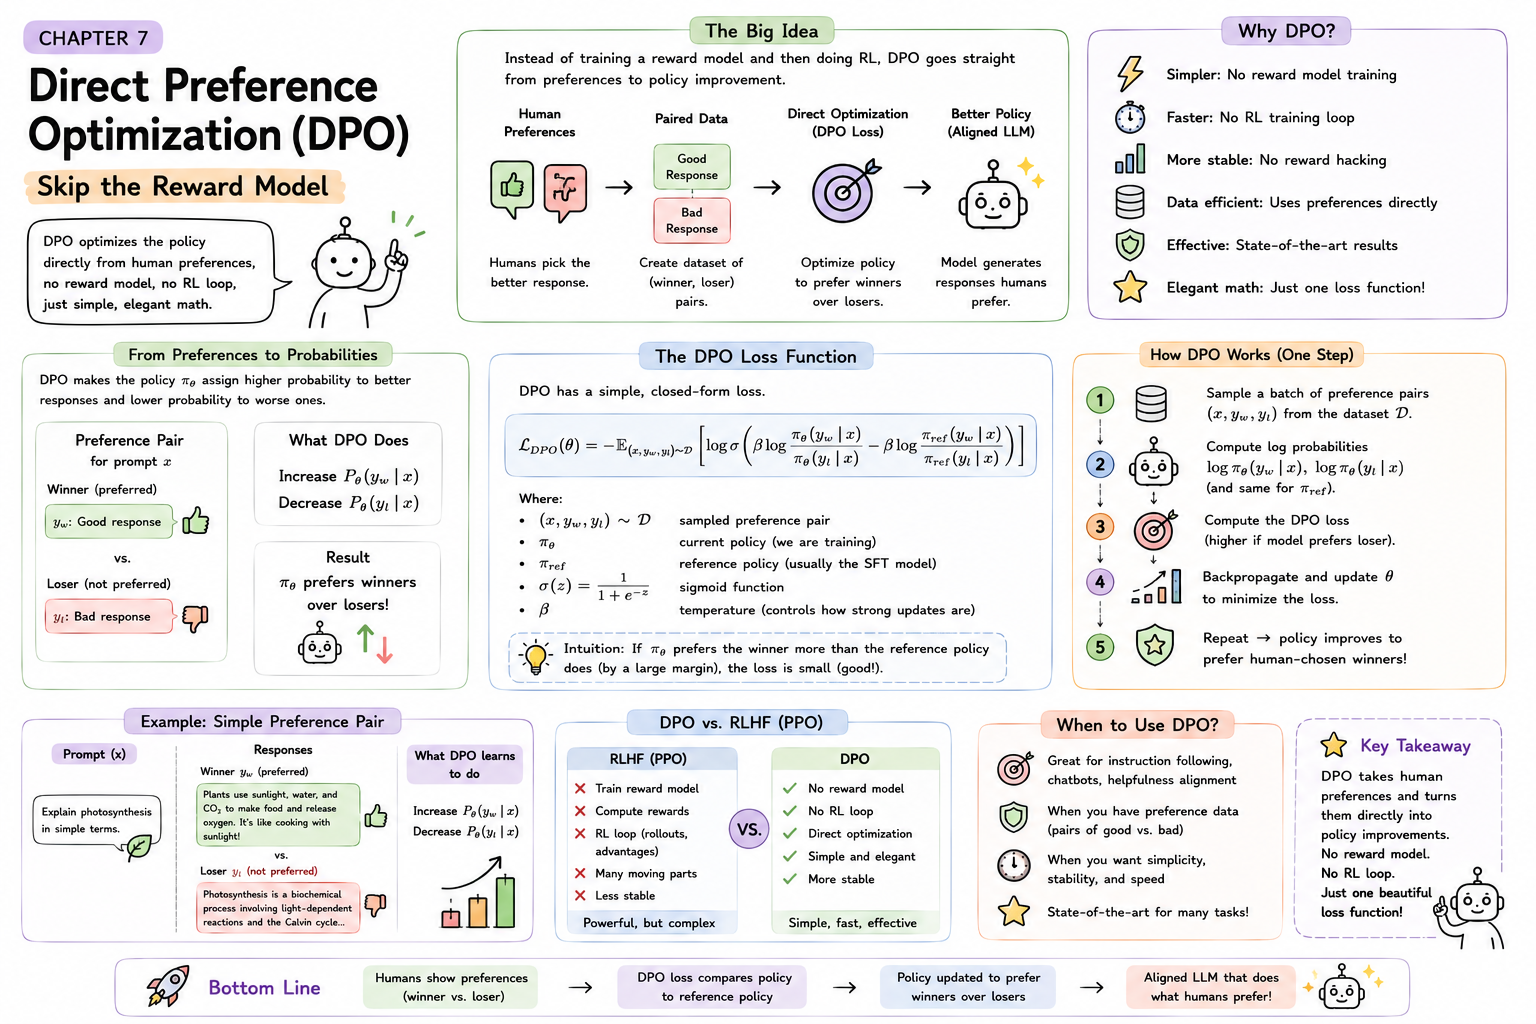
\includegraphics[width=0.88\textwidth]{images/ch07_fig01_dpo_overview.png}
\caption{Direct Preference Optimization at a glance -- skip the reward model, go straight from human preferences to policy improvement with one elegant loss function.}
\label{fig:ch07:dpo_overview}
\end{figure}

\end{chapterenv}